%#!make chemobabel.pdf
%%
%% This document describes the usage of `chemobabel.sty',
%% a LaTeX package for generating chemical structural formulas
%% using Open Babel and Inkscape.
%%
%% Copyright 2014-2022 Acetaminophen (Hironobu YAMASHITA)
%%   Email   :  h.y.acetaminophen[a t]gmail.com
%%   GitHub  :  https://github.com/aminophen
%%   Blog    :  http://acetaminophen.hatenablog.com/
%%   Twitter :  @aminophen
%%
%
\documentclass[12pt]{ltjsarticle}
\usepackage[margin=20mm]{geometry}
\usepackage[english]{babel}
\usepackage[nofontspec,defaultsups]{newpxtext}
\usepackage[zerostyle=c,straightquotes]{newtxtt}
\usepackage{newpxmath}
\usepackage[librsvg]{chemobabel}
\usepackage[bookmarksnumbered=true,hidelinks,%
 pdftitle={User Manual for chemobabel.sty},%
 pdfauthor={Hironobu Yamashita (Acetaminophen)},%
 pdfsubject={TeX \& LaTeX Advent Calendar 2014},%
 pdfkeywords={chemistry,open babel,chemdraw,smiles}]{hyperref}
\usepackage{footnotebackref}
% --- Change the style of captions
% --- (Japanese jsarticle style => English style)
\makeatletter
\long\def\@makecaption#1#2{%
\vskip\abovecaptionskip
\sbox\@tempboxa{#1: #2}
\global\@minipagefalse
\hbox to\hsize{\hfil\box\@tempboxa\hfil}
\vskip\belowcaptionskip}
\makeatother
% --- XyMTeX logo definition
\newcount\TestCount
\def\XyM{\ifnum\fam=-1\relax\fam=0\relax\fi\TestCount=\fam%
X\kern-.30em\smash{\raise.50ex\hbox{$\fam\TestCount\Upsilon$}}%
\kern-.30em{M}}
\def\XyMTeX{\XyM\kern-.1em\TeX}
% ------
\title{\textsf{chemobabel} \\[1ex]
  \normalsize --- Chemical Structures from MDL Molfiles,
  ChemDraw Files or SMILES Notations --- \\
%<ja>  化学構造式をMOLファイルやChemDrawファイル,SMILES表記法から自動生成
  }
\author{Hironobu Yamashita (@aminophen)}
\begin{document}
\renewcommand{\figurename}{Fig.\,}
\pagenumbering{roman}
\maketitle

%<*en>
This document (\jobname.pdf) describes the usage of \textsf{chemobabel.sty},
a \LaTeX\ package for \textbf{generating chemical structural formulas}
to be inserted in your documents.
The formulas can be generated \textbf{from many kinds of chemical data
formats}, including MDL Molfiles, ChemDraw files and even from
SMILES notations, with the help of Open Babel and Inkscape.
The formulas below are generated using this method.

日本語版ドキュメントはchemobabel-ja.pdfを参照してください。
%</en>
%<*ja>
この文書では,\textbf{化学構造式を生成}して\LaTeX の文書中に挿入するための
パッケージである\textsf{chemobabel.sty}と同梱リソースの使い方を説明します。
構造式はOpen Babelの機能を利用することにより,MDL Molfile, ChemDrawファイル,
さらにはSMILES表記法を含む\textbf{さまざまな化学データ形式から生成}できます。
以下の構造式はこの方法によって出力されたものです。

For English documentation, please refer to chemobabel-en.pdf.
%</ja>

\begin{figure}[ht]
  \centering
  \chemobabel[width=65mm]{draw/Firefly luciferin.mol}{} \quad
  \chemobabel[width=90mm]{draw/Brevetoxin A.mol}{}
  \caption{Firefly luciferin \& Brevetoxin A (from MDL Molfiles)}
\end{figure}

\begin{figure}[ht]
  \centering
  \chemobabel[width=90mm]{draw/ATP.cdx}{} \hspace{1cm}
  \chemobabel[width=35mm]{draw/Glucose.cdx}{}
  \caption{ATP (Adenosine triphosphate) \& Glucose (from ChemDraw files)}
\end{figure}

\begin{figure}[ht]
  \centering
  \smilesobabel[width=36mm]{CCO}{} \hspace{1cm}
  \smilesobabel[width=40mm]{CC(C(=O)O)N}{} \hspace{1cm}
  \smilesobabel[width=30mm]{C1[C@H](C)C[C@@H](O)C1}{}
  \caption{Ethanol, Alanine \& (1\textit{S},3\textit{S})-3-Methylcyclopentanol (from SMILES notations)}
\end{figure}

\begin{figure}[ht]
  \centering
  \smilesobabel[width=30mm]{CC(=O)Nc1ccc(cc1)O}{} \hspace{1cm}
  \smilesobabel[width=40mm]{C([C@@H]1[C@H]([C@@H]([C@H]([C@H](O1)O)O)O)O)O}{}
  \caption{Acetaminophen (Paracetamol) \& $\alpha$-\textsc{d}-Glucose (from SMILES notations)}
\end{figure}

\clearpage
\setcounter{tocdepth}{3}
\tableofcontents

\clearpage
\pagenumbering{arabic}

%<*en>
\section{Introduction}
%</en>
%<*ja>
\section{はじめに}
%</ja>

%<*en>
\subsection{Motivation for Development}
%</en>
%<*ja>
\subsection{開発の動機}
%</ja>

%<*en>
As you already know, \LaTeX\ is being used all over the world.
However, when it comes to drawing chemical strucutral formulas,
ways of inserting formulas into \LaTeX\ documents are very limited.
I think it is mainly due to lack of both reliable and simple methods
of doing this that many of the researchers in chemistry are reluctant
to use \LaTeX\ system.
%</en>
%<*ja>
ご存じのとおり,\LaTeX は世界中で使われています。
しかし,化学構造式を描くという点で考えると,
\LaTeX 文書中に構造式を挿入する手段は非常に限られています。
この目的を達成する確実かつ容易な方法が存在しないことは,化学分野における
多くの研究者が\LaTeX システムを使わない要因になっていると考えられます。
%</ja>

%<*en>
Some \TeX/\LaTeX\ macros and packages are already available from
\href{http://www.ctan.org/}{CTAN}:
\begin{itemize}
  \item \href{http://www.ctan.org/pkg/xymtex}{\XyMTeX}:
    a set of packages for drawing chemical structural formulas
\item \href{http://www.ctan.org/pkg/chemfig}{\textsf{chemfig}}:
    a package which draws molecules using Ti\textit{k}Z
\end{itemize}
These packages are reliable and almost all kinds of structural formulas
can be drawn in a consistent way. However, a lot of practice will be
required before one can come to make full use of them.
%</en>
%<*ja>
すでに\href{http://www.ctan.org/}{CTAN}からいくつかのパッケージが利用可能です:
\begin{itemize}
  \item \href{http://www.ctan.org/pkg/xymtex}{\XyMTeX}:
    化学構造式を描くためのパッケージ集
  \item \href{http://www.ctan.org/pkg/chemfig}{\textsf{chemfig}}:
    Ti\textit{k}Zを利用して構造式を描画するパッケージ
\end{itemize}
これらのパッケージは確実で,あらゆる構造式を一貫性をもって描画することができます。
しかし,十分にその機能を活用できるようになるには相当の熟練を要します。
%</ja>

%<*en>
You can also insert structural formulas with \verb|\includegraphics| of
PDF or EPS files exported from special softwares for chemists, such as
\href{http://www.cambridgesoft.com/Ensemble_for_Chemistry/ChemDraw/}{ChemDraw}
and other similar programs.
In this case, you have to save files in both chemical formats
(such as \verb|.cdx| or \verb|.mol|) and graphical formats
(\verb|.pdf| or \verb|.eps|) manually.
%</en>
%<*ja>
化学者向けの専用ツール
(\href{http://www.cambridgesoft.com/Ensemble_for_Chemistry/ChemDraw/}{ChemDraw}など)
でPDFやEPS形式で出力し,\verb|\includegraphics|によって
構造式を取り込むという手段もあります。
この場合,化学用のフォーマット(\verb|.cdx| や \verb|.mol| など)と
画像フォーマット(\verb|.pdf| や \verb|.eps| など)の両方で保存する必要があります。
%</ja>

%<*en>
This new package, \textsf{chemobabel.sty}, will offer a new choice for
chemists who need chemical structures inserted in their \LaTeX\ documents.
In this method, we use \href{http://openbabel.org/}{Open Babel} for
generating chemical structural formulas in SVG format,
and \href{https://inkscape.org/en/}{Inkscape} for converting SVG to PDF.
Both programs are open source and cross-platform, and being actively maintained.
%</en>
%<*ja>
新しいパッケージ \textsf{chemobabel.sty} は,\LaTeX 文書中に化学構造式を
挿入する必要がある化学者に新たな選択肢を提供することでしょう。
この方法では,\href{http://openbabel.org/}{Open Babel}によって
SVG形式の構造式画像を生成し,
さらに\href{https://inkscape.org/ja/}{Inkscape}によってSVGからPDFに変換します。
どちらのプログラムもオープンソースかつクロスプラットフォームであり,
盛んに開発が行われています。
%</ja>

%<*en>
\noindent \textbf{About Open Babel}:

Open Babel is a toolbox specially designed to handle many kinds of
chemical data. It is an open, collaborative project allowing anyone to search,
convert, analyze, or store data from molecular modeling, chemistry,
solid-state materials, biochemistry, or related areas.
See \href{http://openbabel.org/}{Official Website} for detail.
%</en>
%<*ja>
\noindent \textbf{Open Babelについて}

Open Babel はさまざまな化学データを扱うために特別に設計されたツールです。
オープンな共同プロジェクトで,分子モデリング・化学・固体物性・生化学や
関連分野のデータを誰もが検索・変換・分析・保存できることを目指しています。
詳細は\href{http://openbabel.org/}{公式サイト}を参照してください。
%</ja>

\clearpage

%<*en>
\subsection{Idea and Approach}
%</en>
%<*ja>
\subsection{着想とアプローチ}
%</ja>

%<*en>
First I found a post on Noel O'Blog \cite{NOB1}, \cite{NOB2} and
the comment \cite{JLA} about generating chemical structural formulas
from SMILES notations using Open Babel.
I thought the method described in these posts were very interesting,
but I didn't like all the programs could be executed by
\verb|-shell-escape| option.
At the same time, I encountered a macro for copying all
\verb|\includegraphics| from one source file to another \cite{OKU},
which made me conceive of an idea of extracting minimal source code
which needs \verb|-shell-escape| option.

I thought this method would be applicable to converting ChemDraw files into
graphics, but I could not find any project attempting to realize this idea.
I found a project named
\href{http://chemdrawinlatex.sourceforge.net/}{Chemdraw in \LaTeX}
on Sourceforge, but now it was closed.
This drove me to develop a new package to simplify the process for
inserting chemical structural formulas into \LaTeX\ documents.
%</en>

%<*ja>
最初にOpen Babelを用いてSMILES表記から化学構造式を生成するという
Noel O'Blog の記事\cite{NOB1}, \cite{NOB2}とコメント\cite{JLA}を見つけました。
これらの投稿に示された手法は非常におもしろいと思いましたが,
すべてのプログラムが \verb|-shell-escape| オプションによって実行されて
しまうことがあまり好きではありませんでした。
それと同じころ,あるソース中の \verb|\includegraphics| を
別のソースに書き出すというマクロ\cite{OKU}を偶然みつけ,
このとき私は \verb|-shell-escape| が必要な最小のコードだけを抽出する
という着想を得ました。

この方法はChemDrawファイルを画像に変換する目的にも応用できると考えたのですが,
この発想を実現したプロジェクトが見当たらず,ただ一つ見つけたSourceforgeの
\href{http://chemdrawinlatex.sourceforge.net/}{Chemdraw in \LaTeX}は
すでに終了していました。そこで,化学構造式を\LaTeX 文書中に挿入する手順を
簡略化するパッケージを開発しようと考えました。
%</ja>

\clearpage

%<*en>
\section{Before you begin}
%</en>
%<*ja>
\section{パッケージを使う前に}
%</ja>

%<*en>
\subsection{Installing dependent softwares}
%</en>
%<*ja>
\subsection{依存ソフトウェアのインストール}
%</ja>

%<*en>
First, you have to install \href{http://openbabel.org/}{Open Babel} and
\href{https://inkscape.org/en/}{Inkscape}
(or \href{http://librsvg.sourceforge.net/download/}{librsvg}) on your
computer, and export PATH to the command-line binary of both programs,
\verb+obabel+ and \verb+inkscape+ (or \verb+rsvg-convert+).
You can confirm by executing following commands:
%</en>
%<*ja>
初めにコンピュータに\href{http://openbabel.org/}{Open Babel}と
\href{https://inkscape.org/ja/}{Inkscape}(または
\href{http://librsvg.sourceforge.net/download/}{librsvg})をインストールし,
コマンドライン実行ファイルである\verb+obabel+と\verb+inkscape+
(または\verb+rsvg-convert+)にPATHを通します。
正しくPATHが通っているかどうかは以下のコマンドによって確認できます:
%</ja>
%<en>In UNIX operating system:
%<ja>UNIX系の場合:
\begin{verbatim}
$ which obabel
$ which inkscape        (if you choose inkscape)
$ which rsvg-convert    (if you choose librsvg)
\end{verbatim}

%<en>In Windows operating system:
%<ja>Windowsの場合:
\begin{verbatim}
> where obabel
> where inkscape        (if you choose inkscape)
> where rsvg-convert    (if you choose librsvg)
\end{verbatim}

%<*en>
And when you get some command echo, installation should be successful.
%</en>
%<*ja>
何らかのディレクトリ名が返ってきた場合は,正しくインストールできているはずです。
%</ja>

%<*en>
\subsection{Loading the package}
%</en>
%<*ja>
\subsection{パッケージの読み込み}
%</ja>

%<*en>
In the preamble of your document, declare
\begin{verbatim}
\usepackage{chemobabel}
\end{verbatim}
to load \textsf{chemobabel} package.
The package depends on \textsf{graphicx}.
%</en>
%<*ja>
プリアンブルに
\begin{verbatim}
\usepackage{chemobabel}
\end{verbatim}
と宣言して\textsf{chemobabel}パッケージを読み込みます。
これは\textsf{graphicx}パッケージに依存しますので,
もし(u)p\LaTeX を使っていてDVIドライバに\texttt{dvipdfmx}を使用する場合は
ドライバオプション \verb+[dvipdfmx]+ をクラスオプション(グローバル)に
付けるのを忘れないようにしてください。
%</ja>

\clearpage

%<*en>
\section{Basic Usage}
%</en>
%<*ja>
\section{基本的な使い方}
%</ja>
\label{basic}

%<*en>
\subsection{Conversion from Chemical Structure Data Files}
%</en>
%<*ja>
\subsection{化学構造式ファイルからの変換}
%</ja>

%<*en>
Suppose you have \verb|ATP.cdx|, a file with chemical structural formula
of ATP (Adenosine triphosphate) drawn in ChemDraw, and
\verb|Brevetoxin A.mol|, a MDL Molfile which can be obtained from
\href{http://www.chemspider.com/}{ChemSpider} (originally \verb|9041092.mol|).

Use \verb|\chemobabel| command as follows. I put original files in a
subdirectory \texttt{draw}, so added \texttt{draw/} before the actual filename.
Of course you can put in the same directory with your \LaTeX\ file.
%</en>
%<*ja>
\verb|ATP.cdx| はATP(アデノシン三リン酸)の構造式を
ChemDrawで描画したファイル,\verb|Brevetoxin A.mol| は
\href{http://www.chemspider.com/}{ChemSpider}から入手できるファイルです
(もとのファイル名は \verb|9041092.mol| となっています)。

\verb|\chemobabel| コマンドは本文中で以下のようにして使います。
ここでは元のファイルを\texttt{draw}というサブディレクトリに置いたので,
ファイル名の前に \texttt{draw/} を付けました。
もちろん \LaTeX ソースと同一ディレクトリに置くこともできます。
%</ja>

\begin{verbatim}
\chemobabel[width=90mm]{draw/ATP.cdx}{}
\chemobabel[width=120mm]{draw/Brevetoxin A.mol}{}
\end{verbatim}

%<*en>
Then, typeset with \verb|-shell-escape| option.
Remember to use this option, otherwise it won't allow \LaTeX\ to
call any external command-line programs, such as obabel and inkscape!
\begin{verbatim}
$ pdflatex -shell-escape test.tex
\end{verbatim}
You will see in \verb|chemobabelimgdir| subdirectory ``chemobabelimg[NUM].pdf'',
and output file test.pdf will be:
%</en>
%<*ja>
\LaTeX ファイル名がtest.texだとすると,以下のように
\verb|-shell-escape| オプションを与えてタイプセットします。
このオプションを与えることで,\LaTeX が外部プログラムである
obabelやinkscapeを呼んで実行できるようになります。
\begin{verbatim}
$ platex -shell-escape test.tex
\end{verbatim}
すると \verb|chemobabelimgdir| 以下に「chemobabelimg[NUM].pdf」という
ファイルが生成します。得られたtest.dviに対して
\begin{verbatim}
$ dvipdfmx test.dvi
\end{verbatim}
と実行すると,出力される「test.pdf」は以下のようになります:
%</ja>

\begin{figure}[h]
  \centering
  \chemobabel[width=90mm]{draw/ATP.cdx}{} \\ \vspace{1cm}
  \chemobabel[width=120mm]{draw/Brevetoxin A.mol}{}
\end{figure}

%<en>The syntax is:
%<ja>構文は以下のとおりです。
\begin{center}
\verb|\chemobabel[|\textit{options}\verb|]{|\textit{filename}\verb|}{|\textit{obabel options}\verb|}|
\end{center}
%<*en>
As parameters, \textit{filename} should be placed in the first braces, and
\textit{obabel options} (see Section \ref{depict} for some examples)
can be added in the second braces.
You can leave the second parameter empty.

You can give \textit{options} to be passed to \verb|\includegraphics|
command as optional parameters in the box brackets.
This option is not necessary, so can be omitted. In this case the default
option ``scale=1" is passed to \verb|\includegraphics| command.
%</en>
%<*ja>
引数として,中括弧の1つめにファイル名を与え,2つめにobabelに送る
オプション(例は第\ref{depict}節を参照)を指定してください。
2つめの引数は空にすることもできます。

また,オプションとして角括弧に \verb|\includegraphics| に渡すオプションを
指定することができます。
このオプションは省略可能で,何も指定しない場合は scale=1 が適用されます。
%</ja>

%<*en>
\subsection{Conversion from SMILES Notations}
%</en>
%<*ja>
\subsection{SMILES表記法からの変換}
%</ja>

%<*en>
You can also write SMILES notations directly in your \LaTeX\ file to be
converted into structural formulas.
For example, \verb|CCO| is the SMILES notation of ethanol, and
\verb|CC(=O)Nc1ccc(cc1)O| is that of acetaminophen (paracetamol).
Use \verb|\smilesobabel| command as follows:
%</en>
%<*ja>
\LaTeX ソースファイル中に直接SMILES表記を書き込んで,
構造式に変換することもできます。
例えば,\verb|CCO| はエタノールのSMILES表記,
\verb|CC(=O)Nc1ccc(cc1)O| はアセトアミノフェンのSMILES表記です。
\verb|\smilesobabel| コマンドを以下のようにして使います:
%</ja>

\begin{verbatim}
\smilesobabel{CCO}{}
\smilesobabel[width=35mm]{CC(=O)Nc1ccc(cc1)O}{}
\end{verbatim}

%<*en>
Again typeset with \verb|-shell-escape| option:
\begin{verbatim}
$ pdflatex -shell-escape test.tex
\end{verbatim}
This time you will get ``smilesobabelimg[NUM].pdf'' and ``test.pdf'':
%</en>
%<*ja>
やはり \verb|-shell-escape| オプションを付けてタイプセットします。
\begin{verbatim}
$ platex -shell-escape test.tex
$ dvipdfmx test.dvi
\end{verbatim}
すると今度は「smilesobabelimg[NUM].pdf」のようなファイルが生成し,
出力される「test.pdf」は以下のようになります:
%</ja>
\begin{figure}[h]
  \centering
  \smilesobabel{CCO}{} \quad
  \smilesobabel[width=25mm]{CC(=O)Nc1ccc(cc1)O}{}
\end{figure}

%<en>The syntax is:
%<ja>構文は以下のとおりです。
\begin{center}
\verb|\smilesobabel[|\textit{options}\verb|]{|\textit{SMILES notation}\verb|}{|\textit{obabel options}\verb|}|
\end{center}
%<*en>
The only difference from \verb|\chemobabel| is that
\textit{SMILES notation} should be placed in the first braces.
You can put any kinds of SMILES notations in parameters of
\verb|\smilesobabel|, even when they contain some special characters
such as a backslash (\verb|\|) and a percent symbol (\verb|%|).
Similarly, parameters of \verb|\chemobabel| can also contain
these special characters.
%</en>
%<*ja>
\verb|\chemobabel| との唯一の違いは,中括弧の1つめにSMILES表記法の
テキストを与えることだけです。
\verb|\smilesobabel| の引数としては,任意のSMILES表記を用いることができます
(バックスラッシュ (\verb|\|) やパーセント記号 (\verb|%|) のような
特別な文字が入っていてもかまいません)。
なお,\verb|\chemobabel| の引数についても同様に,
特別な文字を含むことができる設計になっています。
%</ja>
\begin{verbatim}
\smilesobabel[width=28mm]{Cl/C=C/Br}{}
\smilesobabel[width=28mm]{Cl/C=C\Br}{}
\end{verbatim}
\begin{figure}[h]
  \centering
  \smilesobabel[width=28mm]{Cl/C=C/Br}{} \quad
  \smilesobabel[width=28mm]{Cl/C=C\Br}{}
\end{figure}

%<*en>
\noindent \textbf{Notes for users of earlier versions} ($\le$ \textsf{chemobabel} v0.6 [2015/06/29])

In earlier versions of \textsf{chemobabel}, it was necessary for users
to pay another attention when using these \LaTeX\ special characters.
However, the workaround I had suggested before was far from desirable
because ``casual \LaTeX\ users'' were forced to change category codes
of these characters manually.

To solve this problem, I prepared supporting macros inside the package
itself ($\ge$ \textsf{chemobabel} v0.7 [2015/08/26]).
Now you can put any kinds of SMILES notations directly without worrying
about special characters (\verb|\|, \verb|%|, etc).
Note that the undesirable workaround (like changing \verb|\catcode| inside
\verb|\begingroup| ... \verb|\endgroup|) has now become rather harmful.
%</en>

%<*ja>
\noindent \textbf{旧バージョンのユーザに対する注意} ($\le$ \textsf{chemobabel} v0.6 [2015/06/29])

古いバージョンの\textsf{chemobabel}では,
これらの\LaTeX で特別な意味を持つ文字に注意を払う必要がありました。
従来私が紹介してきた回避策は“カジュアルな \LaTeX ユーザ”に
カテゴリーコードを手動で変更させていたため,好ましいものではありませんでした。

この問題を解決するため,パッケージ本体の側でこれらの文字をサポートする
マクロを組み込みました(\textsf{chemobabel} v0.7 [2015/08/26] 以降)。
これにより,\verb|\| や \verb|%| といった特別な文字を心配することなく,
任意のSMILES表記を直接引数に渡すことができるようになっています。
従来の回避策(\verb|\begingroup| ... \verb|\endgroup| 内で \verb|\catcode| を
変更する方法)は今ではむしろ有害になっていますので,注意してください。
%</ja>

\clearpage

%<*en>
\subsection{Package options}
%</en>
%<*ja>
\subsection{パッケージオプション}
%</ja>

%<*en>
By default, \textsf{chemobabel} converts chemical structures into
PDF images using Inkscape. However, you can switch the image format
and the conversion program if you like.

When you are using drivers which do not support PDF figures (such as dvips),
it will be helpful if \textsf{chemobabel} converts them into EPS images.
For this purpose, you can use:
%</en>
%<*ja>
\textsf{chemobabel} パッケージは,デフォルトでは化学構造式をInkscapeによって
PDF形式の画像ファイルに変換して文書中に取り込みます。
しかし,オプションで画像形式と変換プログラムを変更することができます。

dvipsなどのPDF非対応のドライバを使用する場合は,EPS形式の画像ファイルに
変換したほうが便利でしょう。この場合
%</ja>
\begin{verbatim}
\usepackage[eps]{chemobabel}
\end{verbatim}
%<*en>
The option \verb|eps| switches the image format (that is, output format
from Inkscape) into EPS ($\ge$ \textsf{chemobabel} v0.9d [2016/02/28]).

You can also change the image conversion program from ``Inkscape'' to
``rsvg-convert'' ($\ge$ \textsf{chemobabel} v0.9e [2016/03/07]).
The program rsvg-convert is faster than inkscape, so it will be useful.
For this purpose, use \verb|librsvg| option:
%</en>
%<*ja>
というように \verb|eps| オプションを指定すれば,内部でInkscapeから出力される
画像形式をPDFではなくEPSに変更します(\textsf{chemobabel} v0.9d [2016/02/28] 以降)。

また,画像変換プログラムを Inkscape から rsvg-convert に変更することもできます
(\textsf{chemobabel} v0.9e [2016/03/07] 以降)。
rsvg-convertはInkscapeより高速ですから,便利かもしれません。
この場合は,以下のように \verb|librsvg| オプションを指定します。
%</ja>
\begin{verbatim}
\usepackage[librsvg]{chemobabel}
\end{verbatim}
%<*en>
The default behavior is equivalent to the \verb|pdf| and \verb|inkscape| options:
%</en>
%<*ja>
デフォルトは \verb|pdf| オプションと \verb|inkscape| オプションを
指定した場合と等価です。
%</ja>
\begin{verbatim}
\usepackage[pdf,inkscape]{chemobabel}
\end{verbatim}

%<*en>
Moreover, Open Babel v2.4.0 or later versions generate images with
a rather large margin. To avoid this, the images are cropped
using \verb|pdfcrop| for PDF or \verb|ps2eps| for EPS
($\ge$ \textsf{chemobabel} v0.9i [2022/09/12]).
If you want to disable this cropping, please add \verb|nocrop| option:
%</en>
%<*ja>
さらに,Open Babel v2.4.0以降で生成される画像はデフォルトで余白が大きいため,
\verb|pdfcrop|(PDFの場合)あるいは\verb|ps2eps|(EPSの場合)で
クロップしています(\textsf{chemobabel} v0.9i [2022/09/12] 以降)。
これをやめたい場合は \verb|nocrop| オプションを指定してください。
%</ja>
\begin{verbatim}
\usepackage[nocrop]{chemobabel}
\end{verbatim}

\clearpage

%<*en>
\subsection{For Safer Typesetting...}
%</en>
%<*ja>
\subsection{安全なタイプセットのために}
%</ja>
\label{extract}

%<*en>
With the basic method described in Section \ref{basic},
you will get desired output in almost any situation.
However, it is sometimes NOT desirable to use \verb|-shell-escape| option,
because with that option \LaTeX\ can call \emph{any} external command-line
programs whether you like it or not.
This means that there is a chance for unknown programs to be executed,
and this can be dangerous especially in case that you don't write your
own \LaTeX\ code. To avoid this problem, I provide a workaround for
extracting all \verb|\chemobabel| and \verb|\smilesobabel| commands
to another \LaTeX\ file (Reference: \TeX\ Forum \cite{OKU}).

All you have to do is to add \verb|extract| option when loading the package:
%</en>
%<*ja>
第\ref{basic}節で述べた基本的な使い方で,ほとんどの場合問題ないでしょう。
しかし,\verb|-shell-escape| オプションを付けてタイプセットするため,
好むと好まざるとにかかわらず\LaTeX が\emph{どんな外部コマンドでも}実行
できてしまいます。つまり,知らないうちにプログラムが実行されてしまう可能性を示唆
しており,これはとりわけ自分で書いた\LaTeX ソースでない場合には危険を伴います。
この問題を回避するために,\verb|\chemobabel| と \verb|\smilesobabel| コマンド
だけを別の \LaTeX ファイルに抽出するマクロを用意しています
(参考:\TeX\ Forum \cite{OKU})。

この場合は,パッケージを読み込む際に \verb|extract| オプションを付与してください。
%</ja>
\begin{verbatim}
\usepackage[extract]{chemobabel}
\end{verbatim}
%<*en>
When typesetting, usual command
\begin{verbatim}
$ pdflatex test.tex
\end{verbatim}
can be used. 
With \verb|extract| option, all \textsf{chemobabel} does is extracting
all \verb|\chemobabel| and \verb|\smilesobabel| commands from the
original \LaTeX\ file.
You will get ``ChemFigFile.tex'' in the same directory, a minimal
\LaTeX\ source file which includes all \verb|\chemobabel| and
\verb|\smilesobabel| commands.
You can simply typeset it by
%</en>
%<*ja>
タイプセットの際には通常の
\begin{verbatim}
$ platex test.tex
\end{verbatim}
というコマンドを使います。
\verb|extract| オプションを付けると,\textsf{chemobabel}パッケージは
単に元の\LaTeX ソースから \verb|\chemobabel| と \verb|\smilesobabel| コマンド
だけを抽出するはたらきをします。
その結果,同じディレクトリに「ChemFigFile.tex」というファイルが生成します。
これは元のソースに書かれていた \verb|\chemobabel| と \verb|\smilesobabel| コマンド
をすべて含む最小の \LaTeX ソースで,これは直接pdflatexでタイプセットできます。
%</ja>
\begin{verbatim}
$ pdflatex -shell-escape ChemFigFile.tex
\end{verbatim}
%<*ja>
欧文と同じ仕様に統一したため,抽出される「ChemFigFile.tex」では
\textsf{graphicx}パッケージに \texttt{[dvipdfmx]} オプション
を与えずに読み込んでいます。したがって,
このタイプセットだけは\texttt{pdflatex}を用いてください。
%</ja>
%<*en>
and you will get PDF figures in the same way
as described in Section \ref{basic}.
After this, typeset your own document again
(this time you should remove \verb|extract| option):
\begin{verbatim}
$ pdflatex test.tex
\end{verbatim}
This time you will get desired output ``test.pdf''
which includes figures properly.
This method will also save you a lot of time for typesetting.
%</en>
%<*ja>
すると,第\ref{basic}節と同様にPDF形式の図のファイルが生成しますので,
あとは \verb|extract| オプションを除去して再度
\begin{verbatim}
$ platex test.tex
$ dvipdfmx test.dvi
\end{verbatim}
と実行すれば,適切に図を取り込んだ望みどおりの「test.pdf」が得られます。
この方法を用いれば,タイプセットに要する時間を大幅に短縮することも期待できます。
%</ja>

\clearpage

%<*en>
\section{Advanced Usage}
%</en>
%<*ja>
\section{高度な使い方}
%</ja>

%<*en>
\subsection{Options for Depiction}
%</en>
%<*ja>
\subsection{描画オプション}
%</ja>
\label{depict}

%<*en>
As I have already mentioned, in both \verb|\chemobabel| and \verb|\smilesobabel|,
you can give some \textit{obabel options} in the second braces.
Here I will introduce some examples.
%</en>
%<*ja>
既に述べたとおり,\verb|\chemobabel| と \verb|\smilesobabel| の両方について,
2つめの中括弧に \textit{obabel options} を与えることができます。
ここで,いくつかの有用な例を挙げておきます。
%</ja>
\begin{itemize}
\item
\begin{verbatim}
\smilesobabel{CC(=O)Nc1ccc(cc1)O}{-xa}
\end{verbatim}
%<en>executes a command which gives a formula with all carbon atoms shown:
%<ja>構造式中の全ての炭素原子を省略せずに描画するコマンドを実行します:
\begin{verbatim}
$ obabel -:"CC(=O)Nc1ccc(cc1)O" -O smilesobabelimg[NUM].svg -xa
\end{verbatim}
\item
\begin{verbatim}
\smilesobabel{CC(=O)Nc1ccc(cc1)O}{-xu -xC}
\end{verbatim}
%<en>gives one without element-specific atom coloring or terminal carbon atoms:
%<ja>元素の着色を行わず,末端の炭素原子を明示しない構造式を出力します:
\begin{verbatim}
$ obabel -:"CC(=O)Nc1ccc(cc1)O" -O smilesobabelimg[NUM].svg -xu -xC
\end{verbatim}
\item
\begin{verbatim}
\chemobabel{ATP.cdx}{-xd}
\end{verbatim}
%<en>You can add \texttt{-xd} option to remove filenames from ChemDraw figures with Open Babel 2.x.
%<ja>Open Babel 2.x系列でChemDrawの図からファイル名を取り除くには,\texttt{-xd} オプションを付けます:
\begin{verbatim}
$ obabel -:"ATP.cdx" -O chemobabelimg[NUM].svg -xd
\end{verbatim}
\end{itemize}

\begin{figure}[ht]
  \centering
  \smilesobabel[width=21mm]{CC(=O)Nc1ccc(cc1)O}{} \hspace{1cm}
  \smilesobabel[width=25mm]{CC(=O)Nc1ccc(cc1)O}{-xa} \hspace{1cm}
  \smilesobabel[width=21mm]{CC(=O)Nc1ccc(cc1)O}{-xu}
  \caption{Acetaminophen (Paracetamol): Nothing, \texttt{-xa}, \texttt{-xu}}
  SMILES: \verb|CC(=O)Nc1ccc(cc1)O|
\end{figure}

\begin{figure}[ht]
  \centering
  \smilesobabel[width=25mm]{C1[C@H](C)C[C@@H](O)C1}{} \hspace{1cm}
  \smilesobabel[width=25mm]{C1[C@H](C)C[C@@H](O)C1}{-xC} \hspace{1cm}
  \smilesobabel[width=25mm]{C1[C@H](C)C[C@@H](O)C1}{-xt}
  \caption{(1\textit{S},3\textit{S})-3-Methylcyclopentanol: Nothing, \texttt{-xC}, \texttt{-xt}}
  SMILES: \verb|C1[C@H](C)C[C@@H](O)C1|
\end{figure}

\begin{figure}[ht]
  \centering
  \smilesobabel[width=42mm]{CCc1cccc(c1)C(=O)Cl}{} \hspace{1cm}
  \smilesobabel[width=42mm]{CCc1cccc(c1)C(=O)Cl}{-xa -xu} \hspace{1cm}
  \smilesobabel[width=42mm]{CCc1cccc(c1)C(=O)Cl}{-xu -xC}
  \caption{3-Ethylbenzoyl chloride: Nothing, \texttt{-xa -xu}, \texttt{-xu -xC}}
  SMILES: \verb|CCc1cccc(c1)C(=O)Cl|
\end{figure}

\begin{figure}[ht]
  \centering
  \smilesobabel[width=42mm]{CCc1cccc(c1)C(=O)Cl}{--highlight "cC=O blue"} \hspace{1cm}
  \smilesobabel[width=42mm]{CCc1cccc(c1)C(=O)Cl}{-xA --genalias}
  \caption{3-Ethylbenzoyl chloride: \texttt{--highlight "cC=O blue"}, \texttt{-xA --genalias}}
  SMILES: \verb|CCc1cccc(c1)C(=O)Cl|
\end{figure}

\begin{figure}[ht]
  \centering
  \chemobabel[width=65mm]{draw/Firefly luciferin.mol}{} \hspace{1cm}
  \chemobabel[width=65mm]{draw/Firefly luciferin.mol}{-xa}
  \caption{Firefly luciferin (from MDL Molfiles): Nothing, \texttt{-xa}}
\end{figure}

\begin{figure}[ht]
  \centering
  \chemobabel[width=70mm]{draw/ATP.cdx}{} \hspace{1cm}
  \chemobabel[width=70mm]{draw/ATP.cdx}{-xd}
  \caption{ATP (from ChemDraw files): Nothing, \texttt{-xd}}
\end{figure}

\begin{figure}[ht]
%<*en>
For more details, see
\href{http://openbabel.org/docs/dev/Command-line_tools/babel.html}{obabel and babel}
and
\href{http://openbabel.org/docs/dev/FileFormats/SVG_2D_depiction.html}{SVG depiction (svg)}
in Open Babel documentation.
%</en>
%<*ja>
より詳細にはOpen Babel documentationの
\href{http://openbabel.org/docs/dev/Command-line_tools/babel.html}{obabel and babel}または
\href{http://openbabel.org/docs/dev/FileFormats/SVG_2D_depiction.html}{SVG depiction (svg)}を
参照してください。
%</ja>
\end{figure}

\clearpage

%<*en>
\subsection{More complex structural formulas}
%</en>
%<*ja>
\subsection{より複雑な構造式}
%</ja>

%<*en>
Open Babel can generate more complex structural formulas from SMILES notations.
%</en>
%<*ja>
Open BabelはSMILES表記から複雑な構造式を生成することができます。
%</ja>

\begin{figure}[ht]
  \centering
  \smilesobabel[width=55mm]{CN1CC[C@]23c4c5ccc(c4O[C@H]2[C@H](C=C[C@H]3[C@H]1C5)O)O}{}
  \caption{($-$)-Morphine}
  SMILES: \verb|CN1CC[C@]23c4c5ccc(c4O[C@H]2[C@H](C=C[C@H]3[C@H]1C5)O)O|
\end{figure}

\begin{figure}[ht]
  \centering
  \smilesobabel[width=150mm]{C[C@@H]1C[C@H]2[C@@H](CC(=O)O2)O[C@H]3C[C@@H]4[C@H](C[C@@H]([C@@H]5[C@@H](O4)C/C=C\C[C@@H]6[C@@H](O5)C/C=C\[C@@H]7[C@@H](O6)CCC[C@@H]8[C@@](O7)(C[C@@H]9[C@@H](O8)C[C@@H]2[C@@H](O9)[C@H](C[C@H](O2)CC(=C)C=O)O)C)C)O[C@@]3(C1)C}{}
  \caption{Brevetoxin A}
  SMILES (Sorry but too long): \verb|C[C@@H]1C[C@H]2[C@@H](CC(=O)O2)O[C@H]3C[C@@H]4[C@H](C[C@@H]([C@@H]5[C@@H](O4)C/C=C\C[C@@H]6[C@@H](O5)C/C=C\[C@@H]7[C@@H](O6)CCC[C@@H]8[C@@](O7)(C[C@@H]9[C@@H](O8)C[C@@H]2[C@@H](O9)[C@H](C[C@H](O2)CC(=C)C=O)O)C)C)O[C@@]3(C1)C|
\end{figure}

%<*en>
However, the results are sometimes undesirable and may also be
different depending on version numbers.
Here are some examples:
%</en>
%<*ja>
しかし,時には結果が望ましくないことがあり,
また使用するバージョン番号によって出力が異なることがあります。
いくつかの例を示します:
%</ja>

\clearpage

\begin{figure}[p]
Cephalostatin-1 (Example from \href{http://en.wikipedia.org/wiki/Simplified_molecular-input_line-entry_system}{Wikipedia}): \\
\verb|C[C@@](C)(O1)C[C@@H](O)[C@@]1(O2)[C@@H](C)[C@@H]3CC=C4[C@]3(C2)C(=O)C[C@H]5[C@H]4CC[C@@H](C6)[C@]5(C)Cc(n7)c6nc(C[C@@]89(C))c7C[C@@H]8CC[C@@H]%10[C@@H]9C[C@@H](O)[C@@]%11(C)C%10=C[C@H](O%12)[C@]%11(O)[C@H](C)[C@]%12(O%13)[C@H](O)C[C@@]%13(C)CO|
\begin{center}
  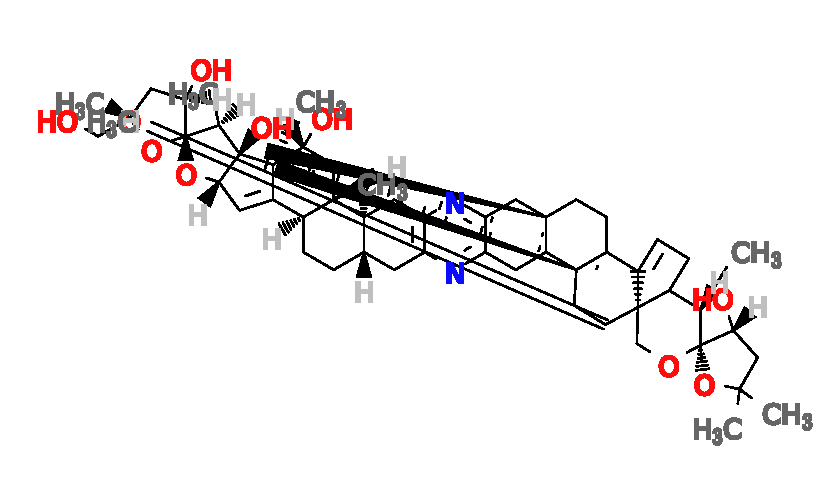
\includegraphics[scale=0.85]{figures/Mac231-Cephalostatin-1.pdf}
  \caption{Cephalostatin-1 (figure from Open Babel for Mac 2.3.1)}
  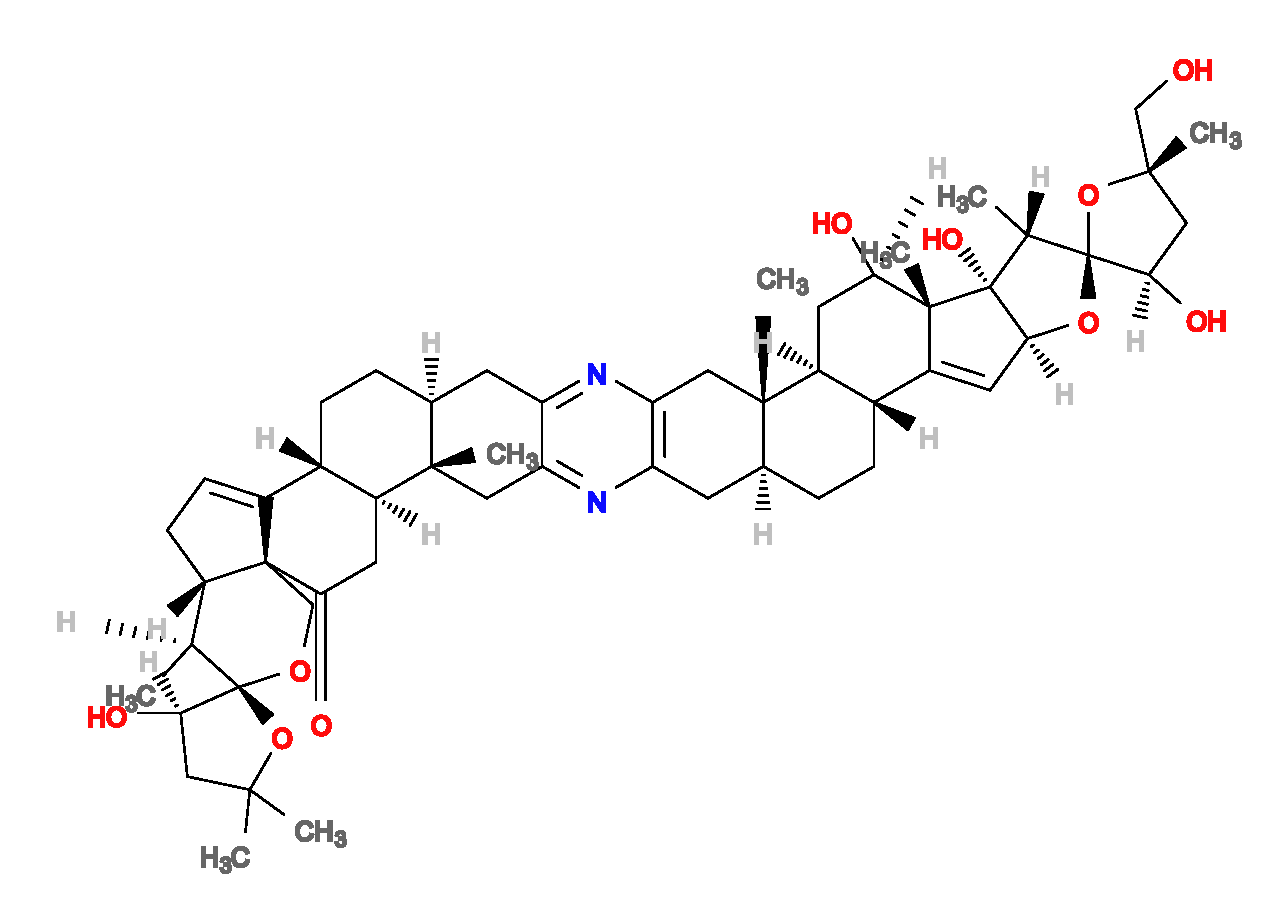
\includegraphics[scale=0.5]{figures/Win232-Cephalostatin-1.pdf}
  \caption{Cephalostatin-1 (figure from Open Babel for Win 2.3.2)}
\end{center}
\end{figure}

\begin{figure}[p]
Sesamin: \verb|c1cc2c(cc1C3C4COC(C4CO3)c5ccc6c(c5)OCO6)OCO2|
\begin{center}
  \centering
  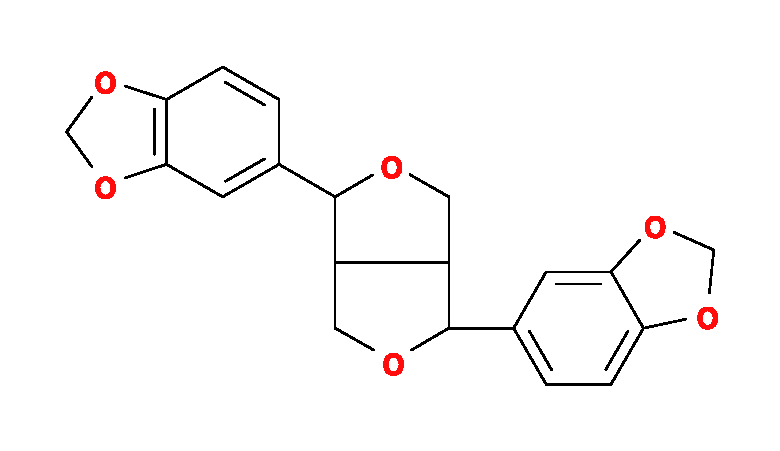
\includegraphics[scale=0.5]{figures/Mac231-sesamin-normal.pdf}
  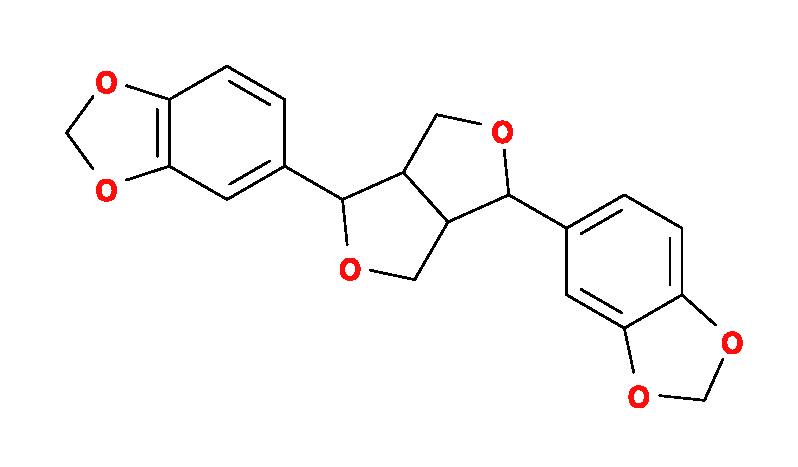
\includegraphics[scale=0.5]{figures/Mac231-sesamin-gen2d.pdf}
  \caption{Sesamin (figures from Open Babel for Mac 2.3.1; Normal and \texttt{--gen2d})}
  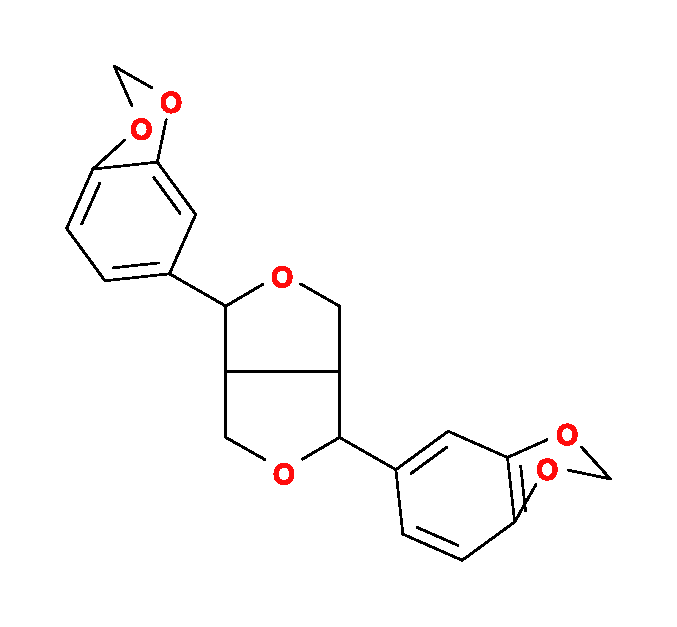
\includegraphics[scale=0.5]{figures/Win232-sesamin-normal.pdf}
  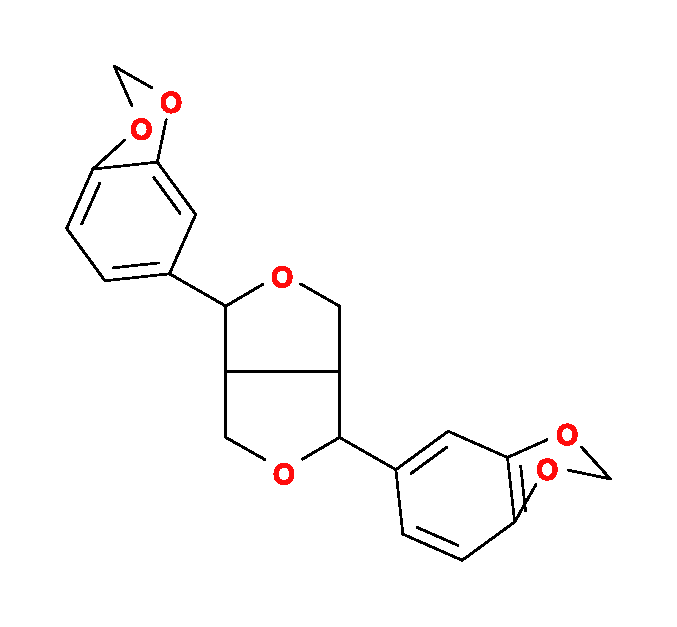
\includegraphics[scale=0.5]{figures/Win232-sesamin-gen2d.pdf}
  \caption{Sesamin (figures from Open Babel for Win 2.3.2; Normal and \texttt{--gen2d})}
\end{center}
\end{figure}

\clearpage

%<*en>
Also, Open Babel may generate wrong structures from SMILES notations.
Here we can see the formula generated from a SMILES notation lacks one double bond.
%</en>
%<*ja>
また,Open BabelはSMILES表記から誤った構造式を生成することもあります。
ホタルルシフェリンの図で,SMILES表記から生成した構造式には
二重結合が一つ欠けています。
%</ja>
\begin{figure}[ht]
  \centering
  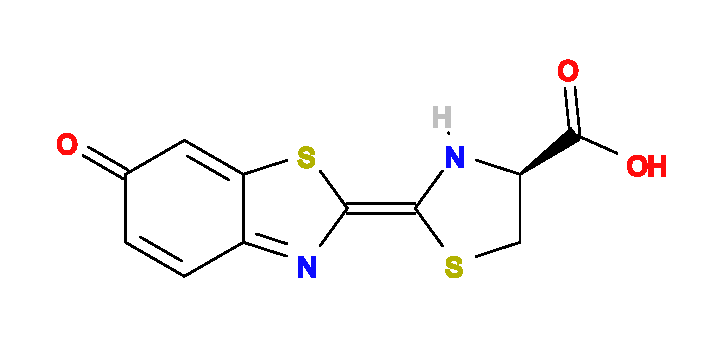
\includegraphics[scale=0.6]{figures/Exact-FireflyLuciferin.pdf}
  \caption{Firefly luciferin: exact structure from ChemSpider ID 4588411}
  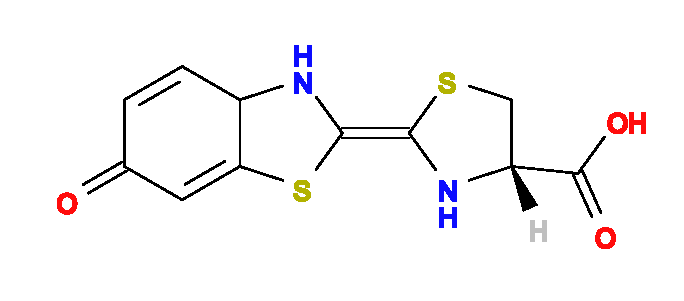
\includegraphics[scale=0.6]{figures/Win232-FireflyLuciferin.pdf}
  \caption{Firefly luciferin?: output from Open Babel for Win 2.3.2}
  \smilesobabel[width=66mm]{C1[C@@H](N/C(=c\2/nc3c(=CC(=O)C=C3)s2)/S1)C(=O)O}{}
  \caption{Firefly luciferin?: output from current Open Babel}
  SMILES: \verb|C1[C@@H](N/C(=c\2/nc3c(=CC(=O)C=C3)s2)/S1)C(=O)O|
\end{figure}

%<*en>
We can avoid all these problems by using \verb|\chemobabel| with \verb|.mol| or
\verb|.cdx| files, instead of \verb|\smilesobabel|.
However, the fact that many complex structures can be generated from
only one character string is very interesting, isn't it?
%</en>
%<*ja>
このような問題点は全て \verb|.mol| または \verb|.cdx| を
用意して \verb|\chemobabel| を利用することで回避できます。
とはいえ,ただの文字列から複雑な構造式を生成しうるということ自体,
おもしろいとは思いませんか?
%</ja>

\clearpage

%<*en>
\section{Note for Compatibility}
%</en>
%<*ja>
\section{互換性に関する注意}
%</ja>

%<*en>
\subsection{Advantages of \textsf{chemobabel}}
%</en>
%<*ja>
\subsection{\textsf{chemobabel}パッケージの有利な点}
%</ja>

%<*en>
The macros \verb|\smiles| (written by Noel O'Boyle \cite{NOB1}) and
\verb|\obabel| (depends on \textsf{graphvizObabel.sty} by
Jakob Lykke Andersen's \cite{JLA}) can be used as follows:
%</en>
%<*ja>
Noel O'Boyleさんによる \verb|\smiles| \cite{NOB1} あるいは
Jakob Lykke Andersenさんによる\textsf{graphvizObabel.sty}が
提供する \verb+\obabel+ \cite{JLA} は以下のようにして使うことになっています:
%</ja>
\begin{verbatim}
% ----- for \smiles command -----
\newcounter{smilescounter}
\setcounter{smilescounter}{1}
\newcommand{\smiles}[1]{
  \immediate\write18{obabel -:"#1" -O smilesimg\arabic{smilescounter}.png}
  \includegraphics{smilesimg\arabic{smilescounter}.png}
  \addtocounter{smilescounter}{1}
}
% ----- for \obabel command -----
\usepackage{graphvizObabel}
% ============ usage ============
\smiles{CCO}
\obabel[scale=0.6]{CCO}
\end{verbatim}
%<*en>
However, \verb|\smiles| command creates raster graphics (.png) and
has no options to pass to \verb|\includegraphics|, and \verb|\obabel| command
sometimes does not work because of lack of file extension (.pdf) and
possibility of giving errors with empty optional parameters.
These problems are solved in \verb|\smilesobabel|.
%</en>
%<*ja>
しかし,\verb|\smiles| はラスター画像 (.png) を生成して
かつ \verb|\includegraphics| に渡すオプションを扱えず,\verb|\obabel| は
拡張子 (.pdf) が欠落していたりオプション引数が空の場合にエラーが発生したり
という理由で正しく処理できない可能性があります。
これらの問題は \verb|\smilesobabel| では解決されています。
%</ja>

\clearpage

%<*en>
\section{Limitations and Alternatives}
%</en>
%<*ja>
\section{この方法の限界と代替案}
%</ja>

%<*en>
This method relies on Open Babel for generating structural formulas,
even without drawing anything by yourself.
Of course you can modify and customize these structures to some extent,
but this method will not be suitable for fine control of the output.
Also, computer-generated formulas may sometimes be unnatural and undesirable.
Therefore this method will be useful only when you need a simple method
for inserting structural formulas with minimal modification.
If you are not satisfied with the output, consider using {\XyMTeX} or
\textsf{chemfig} packages instead.

I also found following packages which can be used for similar purpose:
%</en>
%<*ja>
この方法はOpen Babelに依存して構造式を生成しており,
一切自分で構造式を描画することなく済ませることさえ可能です。
もちろんある程度はそれらの構造を修正したりカスタマイズしたりできますが,
この方法は出力の緻密な調節には不向きでしょう。
また,コンピュータによって生成される構造式は時に見た目が不自然で,
好ましくない場合もあるかもしれません。
したがって,この方法は構造式の出力を完全に制御したいという意図がなく,
構造式を簡便に挿入したい場合にのみ役に立つでしょう。
出力に満足できない場合は,\XyMTeX や\textsf{chemfig}のようなパッケージを
代わりに使うことをご検討ください。

同様の目的を達成するために使えそうなパッケージとして,
以下のようなものもあります:
%</ja>
\begin{itemize}
  \item \href{http://www.ctan.org/pkg/mol2chemfig}{\textsf{mol2chemfig}}:
    convert chemical structures from MDL molfile format
    to \textsf{chemfig} source code
\end{itemize}

\clearpage

%<*en>
\section{Technical information}
%</en>
%<*ja>
\section{技術情報}
%</ja>
\label{detail}

%<*en>
According to
\href{http://www.daylight.com/meetings/summerschool98/course/dave/smiles-intro.html}{SMILES Tutorial},
special characters are used in SMILES syntax are the followings:
%</en>
%<*ja>
SMILES表記法に使われる特殊文字の一覧は,
\href{http://www.daylight.com/meetings/summerschool98/course/dave/smiles-intro.html}{SMILES Tutorial}%
によると以下のようです。
%</ja>
\begin{itemize}
\item Roman alphabets: \verb|A-Z|, \verb|a-z|
\item Numbers: \verb|1-10|
\item Brackets: \verb|[ ] ( )|
\item Others:
\begin{itemize}
\item \verb|*| (unspecified atomic number)
\item \verb|.| (disconnection)
\item \verb|+| (charge sign)
\item \verb|-| (single bond or charge sign)
\item \verb|=| (double bond)
\item \verb|#| (triple bond)
\item \verb|$| (quadruple bond)
\item \verb|:| (aromatic bond)
\item \verb|%| (used when more than 10 ring closures)
\item \verb|/|, \verb|\| (configuration around double bonds)
\item \verb|@| (tetrahedral chirality)
\item \verb|>| (reaction)
\end{itemize}
\end{itemize}

%<*en>
It is important to prevent these characters from being translated as
\LaTeX\ special characters.
However, a backslash (\verb|\|) is a default escape character in \LaTeX,
and a percent symbol (\verb|%|) also has a special meaning as a comment character.
In \textsf{chemobabel} (higher than v0.7), all these characters are
handled properly by changing category codes temporarily (like \verb+\verb+). \\
%</en>
%<*ja>
これらの文字が\LaTeX における特殊文字として解釈されることを防ぐ
必要がありますが,バックスラッシュ \verb|\| はデフォルトの
エスケープ文字であり,またパーセント記号 \verb|%| もコメント文字と
しての特殊な意味を持っています。
\textsf{chemobabel} v0.7以上では,カテゴリーコードを一時的に変更することで
これらすべての文字を適切に扱うようになっています(\verb+\verb+と同様の手法)。
%</ja>

\clearpage

To do (if possible):
\begin{itemize}
\item Check whether \texttt{obabel} and \texttt{inkscape} are successfully
installed or not, before running programs.
\end{itemize}

%<*en>
\section{Version History}
%</en>
%<*ja>
\section{更新履歴}
%</ja>

\begin{table}[h]
\centering
\begin{tabular}{ll}
2014/12/01 v0.1  & Made public as \textsf{smilesobabel.sty} \\
2014/12/02 v0.2  & Add options which can be passed to obabel. \\
2014/12/07 v0.3  & Change name of package: \textsf{chemobabel.sty} \\
                 & Images are stored in \texttt{chemobabelimgdir}. \\
                 & Add \verb|\chemobabel| command. \\
2014/12/09 v0.4  & Fix a bug: (Thanks: Yusuke Terada) \\
                 & Extra spaces at the end of lines are removed. \\
2014/12/20 v0.5  & Add \verb|extract| option. \\
2015/06/29 v0.6  & Improve warning messages. \\
2015/08/26 v0.7  & Solve \verb|\catcode|-related problems in \verb|\smilesobabel|. \\
2015/08/27 v0.8  & Improve \verb|\smilesobabel| a little. \\
2015/08/28 v0.9  & Improve \verb|\smilesobabel|: (Thanks: ZR) \\
                 & Exclude $\varepsilon$-\TeX\ dependency. \\
2015/08/29 v0.9a & Improve \verb|\chemobabel| a little. \\
2016/01/06 v0.9b & Support Lua\TeX-0.85.0 and later versions. \\
2016/02/09 v0.9c & Fix a bug; forgotten in v0.9b. \\
2016/02/28 v0.9d & Add \verb|eps| and \verb|pdf| options. \\
2016/03/07 v0.9e & Add \verb|librsvg| and \verb|inkscape| options. \\
2016/10/23 v0.9f & Incorporate \verb|extract| option into main package. \\
2018/01/23 v0.9g & Minor refactor of code. \\
2022/09/11 v0.9h & Support Inkscape version 1.0 command line syntax. \\
2022/09/12 v0.9i & Crop images before inclusion, add \verb|nocrop| option. \\
2022/09/19 v0.9j & Check shell-escape status to show better error message. \\
\end{tabular}
\end{table}

\textbf{Important!}
\begin{itemize}
\item In Version 0.2, the number of parameters set in \verb|\smilesobabel| is changed!
\item From Version 0.3, the package name is changed to \textsf{chemobabel.sty}.
\item From Version 0.7, the \verb|\catcode|-related workaround is rather harmful.
\end{itemize}

\clearpage

\begin{thebibliography}{9}
\bibitem{NOB1}
\href{http://baoilleach.blogspot.jp/2012/03/cheer-up-your-latex-with-smiles-support.html}{Cheer up your \LaTeX\ with SMILES support} -- Noel O'Blog
\bibitem{NOB2}
\href{http://baoilleach.blogspot.jp/2012/04/cheer-up-your-latex-with-smiles-support.html}{Cheer up your \LaTeX\ with SMILES support II} -- Noel O'Blog
\bibitem{JLA}
\href{http://imada.sdu.dk/~jlandersen/}{\LaTeX: Graphviz and OpenBabel} -- Jakob Lykke Andersen
\bibitem{OKU}
\href{http://oku.edu.mie-u.ac.jp/tex/mod/forum/discuss.php?d=1411}{文章内の画像のみを表示する方法} -- \TeX\ Forum \\
(How to extract only figures in \LaTeX\ source)
\bibitem{ACE1}
\href{http://acetaminophen.hatenablog.com/entry/2014/11/02/130624}{化学構造式を\TeX で(1):自動化による簡単生成} -- Acetaminophen's diary \\
(Chemical Structural Formula in \LaTeX\ (1): An Easy Method by Auto-generation)
\bibitem{ACE2}
\href{http://acetaminophen.hatenablog.com/entry/2014/11/02/130624}{化学構造式を\TeX で(2):自動化の注意点と解消法} -- Acetaminophen's diary \\
(Chemical Structural Formula in \LaTeX\ (2): Important Notes for Auto-generation and Solution)
\bibitem{ACE3}
\href{http://acetaminophen.hatenablog.com/entry/2014/11/05/135927}{化学構造式を\TeX で(3):補足事項} -- Acetaminophen's diary \\
(Chemical Structural Formula in \LaTeX\ (3): Supplement)
\end{thebibliography}

\noindent
\textbf{Note}: \href{http://acetaminophen.hatenablog.com/}{Acetaminophen's diary} is my own blog! (Sorry, but only in Japanese)

I added a post about this package on the 8th day of \href{http://www.adventar.org/calendars/553}{\TeX\ \& \LaTeX\ Advent Calendar 2014} (in Japanese):
\begin{itemize}
\item \href{http://acetaminophen.hatenablog.com/entry/2014/12/08/053519}{誰でも簡単! 化学構造式を\LaTeX に取り込むパッケージ} -- Acetaminophen's diary \\
(An easy way to insert chemical structural formulas into \LaTeX\ documents)
\end{itemize}

\end{document}
